When it comes to interpreting real estate market dynamics, drawing conclusions from data can be more of an art than a science.\cite{Brett2009}

\subsection{The study of complex urban systems, modelling and computation} \label{subsec:study_of_complex_urban_systems_modelling_computation}

An increasing amount of aspects of human life can be traced back through diverse digital footprints and, when aggregated, can reveal emerging patterns.\cite{Arribas-Bel2014}
As such forms of human activity as transactions of land and real estate ownership become digitized\cite{TeranetEnterprisesInc.}, a wealth of data becomes captured and available for analysis.
These increasingly comprehensive archives of human behaviour, combined with the exponential growth of computational power, create potential for transformations in such fields as sociology\cite{Lazer2017} and travel behaviour analysis\cite{Chen2016}.

However, when it comes to using these data sources in social studies, along with opportunities there are also challenges present.
For example, these data sources can have issues with the quality of the data, might require a specific set of skills to take advantage of these data sources, or might not be suitable for traditional methods meant for traditional data\cite{Arribas-Bel2014}.
In addition, when it comes to interpreting real estate market dynamics, drawing conclusions from data can be more of an art than a science.\cite{Brett2009}
Therefore, to study the interaction between land development, urban form, and transportation, it would be beneficial to have a system that can facilitate efficient access to linked information describing these phenomena to researchers from a wide range of disciplines and backgrounds.

The study of complex systems, including urban systems such as land development or transportation, is intrinsically tied to modelling and computation.
Various computer-based models allow us to explore and improve our understanding of the behaviour of a complex system.
Thus, systematic analysis and modelling of urban systems intrinsically depends on our ability to represent and model urban regions and urban processes, which in turn is often limited by our computing software and hardware capabilities.

With large amounts of information about urban regions digitalized\cite{TeranetEnterprisesInc.}, computer-based data storage and data display, manipulation, and management systems, such as Geographic Information Systems (GIS) or Relational Database Management Systems (RDBMS), nowadays play an increasingly important role.
These systems become important because they offer researchers easy access to a wide array of diverse data sources and allow efficient workflows to prepare datasets to be used in statistical analysis software, modelling software, machine learning, etc.


TODO: fuzzy diagram of price

Bourne\cite{Bourne1982} defines urban structure as the combination of the following elements:
\begin{itemize}
    \item urban form, or the spatial configuration of fixed elements within the urban region (including land use, buildings, transportation network, etc.)
    \item urban interactions, or the flows of goods, people, information, and money (including commercial activity, real estate market, etc.)
    \item organizing principles, or the relationships between the urban form and interactions (such as travel cost minimization, social status, segregation, planning policy, etc.)
\end{itemize}


One of the possible ways of studying the interaction between the housing market, urban form, and transportation is empirical, such as examining how property values vary with the distance to a transportation facility\cite{Sherry1999}.
However, this type of research requires fine-scale transportation data to be linked to fine-scale housing market data, which presents a challenge since these data sources use different spatial units (as discussed in section~\ref{sec:spatial_relationships}) and are available at different temporal spans (as discussed in section~\ref{sec:termporal_relationships_between_datasets}).
The primary focus of this mater's thesis is the introduction of a knowledge system providing researchers at the University of Toronto Transportation Research Institute (UTTRI) access to the information required to investigate the complex relationship between transportation and land use.

\subsection{Housing market} \label{subsec:housing_market}

\subsection{Models used for transportation and land use} \label{subsec:transportation_land_use_interaction}


Iacono et al.
\cite{Iacono2008} provide an overview of some of the most common frameworks of Land Use and Transport (LUT) models that have been used to model interaction between transportation and land use in urbanized regions.
Despite the difficulty of modelling of every relevant aspect of an urban region, a wide variety of models were produced dealing with the relationship between transportation network growth and changes in land use and the location of economic activity.
The frameworks can broadly be broken into two major approaches to modelling interactions between land use and transport:
\begin{itemize}
    \item "top-down" modeling frameworks, where interaction between transportation networks and location is specified as a set of aggregate relationships.
    These relationships are based on the behaviour of a representative individual, and are usually taken as a mean calculated from a representative sample of the population.
    These models include:
    \begin{itemize}
        \item aggregate models of spatial interaction
        \item econometric models
    \end{itemize}
    \item "bottom-up" microsimulation models, which cover a number of different approaches to representing the dynamics of land use change and travel behaviour through disaggregating the population and simulating the changes.
    These models include:
    \begin{itemize}
        \item activity-based travel models
        \item multi-agent models
        \item cell-based models
    \end{itemize}
\end{itemize}

% old Teranet challenges

To address these challenges, an efficient and modular Python workflow and a relational database for GTHA housing market are introduced with this master's thesis.
This makes data science methodologies a natural fit when trying to get a deeper understanding of the nature of "wicked" urban problems, such as the interaction between land development, urban form, and transportation.

\subsection{Data quality, skill requirements and lack of features} \label{subsec:challenges_quality_skills_features}

Teranet dataset presents an extensive historical record of real estate transactions recorded in the Province of Ontario since the beginning of XIX century.
However, when it comes to using new data sources in social studies, along with opportunities there are also challenges present.
For example, these data sources can have issues with the quality of the data, might require a specific set of skills to take advantage of these data sources, or might not be suitable for traditional methods meant for traditional data\cite{Arribas-Bel2014}, all of which are true in the case of Teranet's dataset.

On top of the issues with Teranet's data mentioned above, the most significant challenge lies in the amount of features provided for each record.
Despite capturing effectively the complete population of real estate transactions recorded in Ontario since 1985, the available version of the dataset includes no information describing anything about each transaction, other than its location in the form of address and coordinates, the registration date, and the consideration amount.
Since is no distinction being made between transactions recorded for residential, commercial, and industrial property types, transaction amounts can vary from several dollars to billions of dollars.
There are no attributes that would allow transactions to be filtered for meaningful analysis and modeling.

\subsection{Size of datasets, computational requirements and file formats} \label{subsec:challenges_size_and_formats}

To address this gap, additional attributes can be joined from various data sources, such as Census, TTS or land use data, based on spatial or temporal relationships.
However, Teranet's dataset has a number of records on the order of $10^6$.
Such data sources as Census tables have the number of fields on the order of $10^2$.
Overall, the number of attributes that could be joined between the various available data sources will probably be on the order of $10^3$.
This fact makes it increasingly impractical to store all the data in one table, due to the memory requirements for storage and processing.

In addition, datasets coming from different sources arrive in different file formats, such as text files, Excel spreadsheets, .csv files, or shapefiles.
Combined with the size of the datasets and the computational requirements of such processing techniques as spatial joins, the facts mentioned above make working with Teranet's difficult due to the hardware and special skill requirements.

\subsection{Complex spatial and temporal relationships between urban data sources} \label{subsec:complex_spatio-temporal_relationships_between_urban_data_sources}

%TODO write subsection

\subsection{The proposed solution: Python-SQL back-end} \label{subsec:proposed_solution_python_sql_backend}

To address this challenge, this master's thesis establishes an organized modular data preparation workflow for Teranet's dataset and other related data sources and organized them into a relational database.
A Relational Database Management System (RDBMS), such as PostgreSQL, will deliver the benefit of organized and optimized data storage, access, and processing;
it is also capable of facilitating the flexibility and modular structure that is dictated by the nature of the data sources and the scope of research activities undertaken by UTTRI .
The data preparation workflow is facilitated via Python in a series of jupyter notebooks described in section \textbf{cite}
%TODO rewrite proposed solution to ML workflow

\subsection{Accessibility as a measure of land use-transportation relationship} \label{subsec:accessibility}

While transportation research started as an isolated field focusing on mobility, researchers recognized that trips are made to access particular destinations\cite{VanLierop2017}.
A concept of accessibility, understood as the ease of reaching rather than simply the ease of moving\cite{Preston2007}, was developed to take into account the location of urban opportunities.
Accessibility is the mediating factor between the location of activities and demand for travel and is discussed further in section~\ref{subsec:accessibility} of the following chapter.

LUT models (discussed in section~\ref{subsec:transportation_land_use_interaction}) operationalize the transportation-land use relationship by incorporating measures of accessibility with the process of locating activities, typically assuming that households wish to locate in areas with higher accessibility to employment, shopping, or entertainment opportunities.
Similarly, firms are assumed to locate in areas with higher accessibility to labour markets.
Land use component is usually integrated into the accessibility measure through congested network travel times.
However, when studying the relationship between transportation facilities and property values, results may vary based on whether travel time or travel distance is used as a measure of accessibility\cite{Sherry1999}.

Accessibility measures the situation of a location relative to other activities or opportunities (work, shopping, etc.) distributed in space and can be an important determinant of price in LUT models where land and floor space markets are considered explicitly\cite{Iacono2008}.
When measuring changes in relative accessibility, it is usually approximated by some measure of access to the transportation network, such as travel time or distance.

Economic decisions made by the households and firms act as one of the links between the tranportation and land use systems.
When choosing a location, households and firms attempt to fulfill as many of their location preferences as possible while facing constraints.
One of the main constraints is the price or rent of the dwelling, related to the income of the household;
another important constraint is travel time, with suitable location being restricted by the travel times and transportation expenses\cite{Moeckel2017}.

On the purchase and sale of real estate and land, ownership is generally transferred to the buyer when the deed or transfer is registered in the applicable land registry office.
An agreement of purchase and sale must be in writing to be enforceable.
A transfer of ownership is actualised by registering, either physically or electronically (depending on the applicable land registry system), a deed or transfer with the applicable land registry office or land registrar.

However, along with opportunities, there are also challenges present.
Teranet's dataset of land registration records presents a wealth of information about the housing market at a very fine scale but is severely limited in the number of features describing each transaction.
One of the main features that is missing is the type of property being transacted (e.g., single detached house, apartment/condo, commercial, mix use, etc.).
Teranet's dataset and the main challenges of using it for ILUTE improvement and Longitudindal Housing Market Research, along with the proposed solution, is discussed in section~\ref{sec:new_data_sources_and_their_challgenges}.

\subsection{ILUTE model system and HoMES} \label{subsec:ilute_and_homes}

The system state is defined in terms of the individual persons, households, dwelling units, firms, etc.
that collectively define the urban region being modeled\cite{Miller2011}.
The model aims to capture the dynamics of these markets through disaggregated representations.
For example, in the housing market component of ILUTE, houses are auctioned off one dwelling at a time to interested bidders in a disaggregate implementation of Martinez' Bid Choice theory\cite{Martinez1992}.

The ILUTE model system simulates the evolution of an urban region's spatial form, demographics, travel behavior and economic structure over time.
The model aims to capture the dynamics of these markets through disaggregated representations.

The Housing Market Evolutionary System (HoMES) is the updated housing market module for the ILUTE model system.
HoMES is a disaggregate, agent-based microsimulation of the owner-occupied housing market that evolves the residential location of households over time and includes the endogenous supply of housing by type and location, as well as the endogenous determination of sales prices and rents.

An overview of the framework of housing market supply, demand and clearing mechanisms utilized in HoMES provided by Rosenfield et al.\cite{Rosenfield2013} is presented on figure~\ref{fig:homes_framework}
\begin{figure}[hbt!]
    \centering
    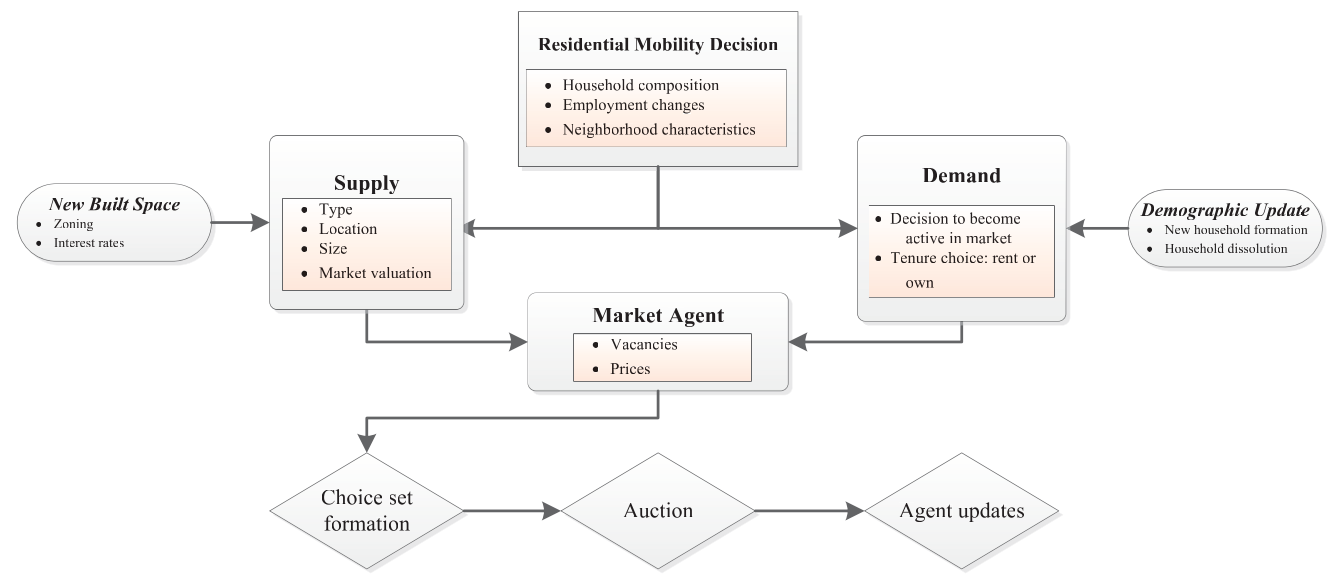
\includegraphics[width=0.99\linewidth,trim=0 0 0 0,clip]{homes_framework.png}
    \caption{Framework of housing market supply, demand and clearing mechanisms used in HoMES module of ILUTE, as summarized by Rosenfield et al.\cite{Rosenfield2013}.}
    \label{fig:homes_framework}
\end{figure}

In the case of ILUTE and HoMES, one of the possibilities for further improvement is the use of new data sources to update the housing market model.
One of these new data sources is Teranet's dataset of land registry records;
its background, challenges and the proposed solution are discussed in the remainder of this chapter.

Changes to relative accessibility of a location can thus be estimated as changes in zone-to-zone travel times in a travel network\cite{Iacono2008}.


The proposed GTHA housing market database combines urban data coming from a variety of sources.
At the heart of it lies Teranet's dataset of real estate transactions (land registration records) recorded in the Province of Ontario since the beginning of XIX century up to October of 2017.




As defined by Codd (\cite{Codd1990}, section 17.5.1), the basic ideas in normalization are to organize the information in a database as follows:

\begin{enumerate}
    \item Each distinct type of object has a distinct type identifier, which becomes the name of a base relation.
    \item Every distinct object of a given type must have an instance identifier that is unique within the object type;
    this is called its primary-key value.
    \item Every fact in the database is a fact about the object identified by the primary key.
    \item Each such fact contains nothing other than the single-valued immediate properties of the object.
    \item Such facts are collected together in a single relation, if they are about objects of the same type.
    The result is a collection of facts, all of the same type.
\end{enumerate}

According to Wickham, the most common problems with messy datasets are:
\begin{itemize}
    \item Column headers are values, not variable names.
    \item Multiple variables are stored in one column.
    \item Variables are stored in both rows and columns.
    \item Multiple types of observational units are stored in the same table.
    \item A single observational unit is stored in multiple tables.
\end{itemize}

% Alternative abstract


Microsimulation models are the latest generation of models used to study the complex interaction of land use and transportation;
these models use highly disaggregated representation of markets and processes.
Increased digitization of human activity produced new data sources that offer higher spatial and temporal resolution, making them valuable for design and validation of urban models.
Introduction of the POLARIS system in Ontario in 1985 lead to the creation of an extensive dataset of land registration records, capturing every property sale in Ontario.
However, despite the high resolution, Teranet's dataset suffers from the lack of features characterizing each transaction, most notably, the type of the property being sold.
This master's thesis proposes a prototype of a workflow to augment Teranet's dataset with data from multiple sources and use machine learning to classify land use at transaction level based on the housing market dynamics.
